% Reset frame number to 1
\setcounter{framenumber}{0}

% Section title slide
\begin{frame}
\frametitle{Linear Regression}
\begin{center}
\Large \textbf{Linear Regression}
\end{center}
\end{frame}

\section{Linear Regression}

\begin{frame}{Motivation: Why Linear Regression?}
  \begin{itemize}
    \item Foundational model for supervised learning and statistical inference.
    \item Interpretable parameters with clear geometric meaning.
    \item Lays the foundation for building ML models.
    \item Later supports building neural networks (linear layers).
    \item Efficient algorithms with both closed-form and iterative solutions.
  \end{itemize}
\end{frame}

\begin{frame}{Learning Objectives}
  By the end of this lecture, you should be able to:
  \begin{itemize}
    \item Formulate linear regression in scalar and vectorized forms.
    \item Define and analyze the MSE loss.
    \item Derive gradients and apply gradient descent variants.
    \item Compute the closed-form solution and understand its limitations.
    \item Extend linear regression via features and regularization.
  \end{itemize}
\end{frame}

\begin{frame}{Supervised Learning: Formal Definition}
  \begin{block}{Setup}
    Given labeled data
    \[
      \mathcal{D} = \{(\mathbf{x}^{(i)}, y^{(i)})\}_{i=1}^m, \quad \mathbf{x}^{(i)} \in \R^n, \; y^{(i)} \in \R,
    \]
    learn a hypothesis \(h_{\boldsymbol{\theta}}\) that predicts \(y\) from \(\mathbf{x}\).
  \end{block}
  \begin{itemize}
    \item Hypothesis class: \( \mathcal{H} = \{h_{\boldsymbol{\theta}} : \boldsymbol{\theta} \in \R^{n+1}\}\)
    \item Loss function \( \ell(h_{\boldsymbol{\theta}}(\mathbf{x}), y) \) measures prediction error.
  \end{itemize}
\end{frame}

\begin{frame}{Supervised Learning Pipeline}
  \begin{enumerate}
    \item Curate labeled data \( \{(\mathbf{x}^{(i)}, y^{(i)})\}_{i=1}^m \).
    \item Choose a hypothesis class and parameters \( \boldsymbol{\theta} \).
    \item Define a loss function (e.g., MSE).
    \item Learn by minimizing empirical risk (loss on training data).
  \end{enumerate}

\end{frame}

\begin{frame}{Training vs.\ Test Error}
  \begin{itemize}
    \item \textbf{Training error}: loss on the dataset used for fitting.
    \item \textbf{Test error}: loss on unseen data from the same distribution.
    \item \textbf{Generalization gap}: difference between train and test error.
  \end{itemize}
  \begin{block}{Goal}
    Minimize training loss
    \[
      \mathcal{L}(\boldsymbol{\theta}) = \frac{1}{m} \sum_{i=1}^m \ell(h_{\boldsymbol{\theta}}(\mathbf{x}^{(i)}), y^{(i)}).
    \]
  \end{block}

  \vspace{0.5em}
  \textbf{Key point:}
  \[
    \mathcal{L}(\boldsymbol{\theta}) \neq \mathcal{L}(\boldsymbol{\theta}^*)
  \]
\end{frame}

\begin{frame}{Running Example: Simple Linear Regression}
  Model:
  \[
    y = \theta_0 + \theta_1 x
  \]
  \begin{itemize}
    \item \(\theta_0\): intercept, \(\theta_1\): slope.
    \item Captures linear trend between input and output.
  \end{itemize}
\end{frame}

\begin{frame}{Observation Noise}
  \[
    y = \theta_0 + \theta_1 x + \varepsilon, \quad \varepsilon \sim \mathcal{N}(0, \sigma^2)
  \]
  \begin{itemize}
    \item Noise models unobserved factors and measurement error.
    \item Leads to probabilistic interpretation of least squares.
  \end{itemize}
\end{frame}

\begin{frame}{Synthetic Data Visualization}
  \centering
  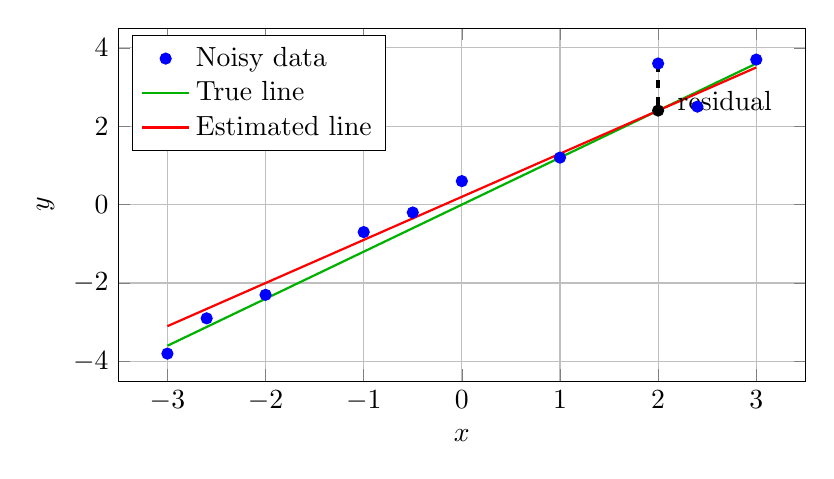
\begin{tikzpicture}
    \begin{axis}[
      width=0.85\textwidth,
      height=0.5\textwidth,
      xlabel={$x$},
      ylabel={$y$},
      xmin=-3.5, xmax=3.5,
      ymin=-4.5, ymax=4.5,
      legend style={at={(0.02,0.98)},anchor=north west},
      legend cell align=left,
      grid=major
    ]
      \addplot[only marks, mark=*, color=blue] coordinates {
        (-3,-3.8)
        (-2,-2.3)
        (-1,-0.7)
        (0,0.6)
        (1,1.2)
        (2,3.6)
        (3,3.7)
        (-2.6,-2.9)
        (-0.5,-0.2)
        (2.4,2.5)
      };
      \addlegendentry{Noisy data}
      \addplot[domain=-3:3, samples=2, thick, color=green!70!black] {1.2*x};
      \addlegendentry{True line}
      \addplot[domain=-3:3, samples=2, thick, color=red] {0.2 + 1.1*x};
      \addlegendentry{Estimated line}

      % Residual annotation
      \addplot[very thick, dashed, color=black] coordinates {(2,3.6) (2,2.4)};
      \addplot[mark=*, color=black] coordinates {(2,2.4)};
      \node[anchor=west] at (axis cs:2.1,2.65) {residual};
    \end{axis}
  \end{tikzpicture}
\end{frame}

\begin{frame}{From Simple to General Linear Regression}
  For \(n\)-dimensional inputs:
  \[
    y = \theta_0 + \theta_1 x_1 + \cdots + \theta_n x_n
  \]
  \begin{itemize}
    \item Each feature contributes linearly to the prediction.
    \item Still linear in parameters \(\boldsymbol{\theta}\).
  \end{itemize}
\end{frame}

\begin{frame}{Vectorized Representation}
  Introduce dummy feature \(x_0 = 1\):
  \[
    y = \boldsymbol{\theta}^T \mathbf{x}, \quad \mathbf{x} = [x_0, x_1, \ldots, x_n]^T
  \]
  Dimensions:
  \[
    \mathbf{x} \in \R^{n+1}, \quad \boldsymbol{\theta} \in \R^{n+1}
  \]
\end{frame}

\begin{frame}{Dataset in Matrix Form}
  Stack examples into a matrix:
  \[
    X \in \R^{m \times (n+1)}, \quad \mathbf{y} \in \R^m
  \]
  Predictions:
  \[
    \hat{\mathbf{y}} = X\boldsymbol{\theta}
  \]
\end{frame}

\begin{frame}{Mean Squared Error (MSE)}
  \[
    \mathcal{L}(\boldsymbol{\theta}) = \frac{1}{m} \sum_{i=1}^m \left(y^{(i)} - \boldsymbol{\theta}^T \mathbf{x}^{(i)}\right)^2
  \]
  \begin{itemize}
    \item Penalizes large errors more strongly.
    \item Smooth, convex, and easy to optimize.
  \end{itemize}
\end{frame}

\begin{frame}{Why Squared Loss?}
  \begin{itemize}
    \item Maximum likelihood estimator under Gaussian noise.
    \item Differentiable and convex.
    \item Leads to closed-form solutions.
  \end{itemize}
  \[
    p(y \mid \mathbf{x}, \boldsymbol{\theta}) = \mathcal{N}(\boldsymbol{\theta}^T \mathbf{x}, \sigma^2)
  \]
\end{frame}

\begin{frame}{Learning as Optimization}
  Empirical risk minimization:
  \[
    \min_{\boldsymbol{\theta}} \; \mathcal{L}(\boldsymbol{\theta})
  \]
  \begin{itemize}
    \item \(\mathcal{L}(\boldsymbol{\theta})\) is a convex quadratic.
    \item Unique minimizer if \(X^T X\) is full rank.
  \end{itemize}
\end{frame}

\begin{frame}{Geometry of Least Squares}
  \begin{itemize}
    \item Column space of \(X\) defines all possible predictions.
    \item Optimal \(\hat{\mathbf{y}}\) is orthogonal projection of \(\mathbf{y}\) onto \(\text{col}(X)\).
    \item Residual \(\mathbf{r} = \mathbf{y} - X\boldsymbol{\theta}^*\) satisfies \(X^T \mathbf{r} = 0\).
  \end{itemize}
\end{frame}

\begin{frame}{Gradient of the MSE Loss}
  \[
    \nabla_{\boldsymbol{\theta}} \mathcal{L}(\boldsymbol{\theta}) = \frac{2}{m} X^T (X\boldsymbol{\theta} - \mathbf{y})
  \]
  \begin{itemize}
    \item \(X\boldsymbol{\theta} - \mathbf{y}\): residual vector.
    \item \(X^T\): aggregates residuals by feature.
  \end{itemize}
\end{frame}

\begin{frame}{What Is a Gradient?}
  \begin{itemize}
    \item Gradient is a vector of partial derivatives:
      \[
        \nabla_{\boldsymbol{\theta}} \mathcal{L}(\boldsymbol{\theta})
        = \left[\frac{\partial \mathcal{L}}{\partial \theta_0}, \ldots,
        \frac{\partial \mathcal{L}}{\partial \theta_n}\right]^T
      \]
    \item Points in the direction of steepest ascent.
    \item The negative gradient gives the direction of steepest descent.
  \end{itemize}
  \[
    \mathcal{L}(\boldsymbol{\theta} + \Delta) \approx \mathcal{L}(\boldsymbol{\theta}) + \nabla_{\boldsymbol{\theta}} \mathcal{L}(\boldsymbol{\theta})^T \Delta
  \]
\end{frame}

\begin{frame}{Gradient Descent Update Rule}
  Iterative update (move opposite the gradient):
  \[
    \boldsymbol{\theta}^{(t+1)} = \boldsymbol{\theta}^{(t)} - \eta \nabla_{\boldsymbol{\theta}} \mathcal{L}(\boldsymbol{\theta}^{(t)})
  \]
  \begin{itemize}
    \item \(\eta > 0\) is the step size (learning rate).
    \item Larger gradient \(\Rightarrow\) larger update direction.
  \end{itemize}
\end{frame}

\begin{frame}{Choosing the Step Size}
  \begin{itemize}
    \item \textbf{Too small}: very slow convergence.
    \item \textbf{Too large}: divergence or oscillation.
    \item Practical strategies:
      \begin{itemize}
        \item Start with a moderate \(\eta\) and tune on validation loss.
        \item Use decaying schedules: \(\eta_t = \eta_0 / (1 + \alpha t)\).
        \item Normalize features to reduce conditioning issues.
      \end{itemize}
  \end{itemize}
\end{frame}

\begin{frame}{Convergence and Conditioning}
  \begin{itemize}
    \item Quadratic objectives allow linear convergence rates.
    \item Poorly conditioned \(X^T X\) slows convergence.
    \item Feature scaling can dramatically improve speed.
  \end{itemize}
\end{frame}

\begin{frame}{Pros and Cons of Gradient Descent}
  \textbf{Pros}
  \begin{itemize}
    \item Scales to large datasets.
    \item Works with regularized and non-closed-form objectives.
  \end{itemize}
  \textbf{Cons}
  \begin{itemize}
    \item Requires step-size tuning.
    \item For nonconvex losses, may converge to local minima or saddle points.
  \end{itemize}
  \vspace{0.3em}
  \textbf{Note:} Linear regression is convex, so GD converges to the global optimum.
\end{frame}

\begin{frame}{Gradient Descent Pseudocode}
  \begin{algorithm}[H]
  \SetAlgoLined
  \KwIn{Data matrix $X$, targets $\mathbf{y}$, step size $\eta$, iterations $T$}
  \KwOut{Parameters $\boldsymbol{\theta}$}
  Initialize $\boldsymbol{\theta} \leftarrow 0$\;
  \For{$t=1$ \textbf{to} $T$}{
    $g \leftarrow \frac{2}{m} X^T (X\boldsymbol{\theta} - \mathbf{y})$\;
    $\boldsymbol{\theta} \leftarrow \boldsymbol{\theta} - \eta g$\;
  }
  \end{algorithm}
\end{frame}

\begin{frame}{Gradient Descent Visualization}
  \centering
  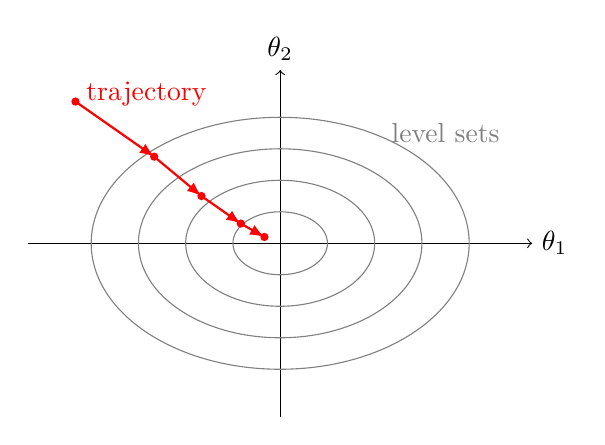
\begin{tikzpicture}
    \draw[->] (-3.2,0) -- (3.2,0) node[right] {$\theta_1$};
    \draw[->] (0,-2.2) -- (0,2.2) node[above] {$\theta_2$};

    % Contours of a quadratic loss (ellipses)
    \draw[gray] (0,0) ellipse (0.6 and 0.4);
    \draw[gray] (0,0) ellipse (1.2 and 0.8);
    \draw[gray] (0,0) ellipse (1.8 and 1.2);
    \draw[gray] (0,0) ellipse (2.4 and 1.6);

    % Optimization trajectory
    \draw[red, thick, -latex] (-2.6,1.8) -- (-1.6,1.1);
    \draw[red, thick, -latex] (-1.6,1.1) -- (-1.0,0.6);
    \draw[red, thick, -latex] (-1.0,0.6) -- (-0.5,0.25);
    \draw[red, thick, -latex] (-0.5,0.25) -- (-0.2,0.08);
    \fill[red] (-2.6,1.8) circle (1.5pt);
    \fill[red] (-1.6,1.1) circle (1.5pt);
    \fill[red] (-1.0,0.6) circle (1.5pt);
    \fill[red] (-0.5,0.25) circle (1.5pt);
    \fill[red] (-0.2,0.08) circle (1.5pt);

    \node[gray] at (2.1,1.4) {level sets};
    \node[red] at (-1.7,1.9) {trajectory};
  \end{tikzpicture}
\end{frame}

\begin{frame}{Variants of Gradient Descent}
  \begin{itemize}
    \item \textbf{Batch GD}: uses all data per update.
    \item \textbf{Stochastic GD}: uses one example at a time.
    \item \textbf{Mini-batch GD}: uses small batches.
  \end{itemize}
  Trade-offs: computation vs.\ variance vs.\ convergence speed.
\end{frame}

\begin{frame}{GD Variants: Gradient Estimates}
  Let \(\mathcal{B}_t\) be a batch at iteration \(t\).
  \[
    g_t = \frac{2}{|\mathcal{B}_t|} X_{\mathcal{B}_t}^T (X_{\mathcal{B}_t}\boldsymbol{\theta} - \mathbf{y}_{\mathcal{B}_t})
  \]
  \begin{itemize}
    \item Batch GD: \(\mathcal{B}_t = \{1,\ldots,m\}\), low variance, high cost.
    \item SGD: \(|\mathcal{B}_t| = 1\), high variance, fast iterations.
    \item Mini-batch: \(1 < |\mathcal{B}_t| \ll m\), best of both.
  \end{itemize}
\end{frame}

\begin{frame}{Practical Notes on GD Variants}
  \begin{itemize}
    \item Shuffle data each epoch to avoid bias in SGD.
    \item Use momentum or adaptive methods (Adam) for faster training.
    \item Larger batches suit parallel hardware; smaller batches generalize well.
  \end{itemize}
\end{frame}

\begin{frame}{When to Use Which Variant}
  \begin{itemize}
    \item Small \(m\): Batch GD is efficient and stable.
    \item Large \(m\): Mini-batch for parallelism and speed.
    \item Streaming data: Stochastic/online updates.
  \end{itemize}
\end{frame}

\begin{frame}{Closed-Form Solution: Normal Equations}
  Solve \(\nabla_{\boldsymbol{\theta}} \mathcal{L}(\boldsymbol{\theta}) = 0\):
  \[
    X^T X \boldsymbol{\theta} = X^T \mathbf{y}
  \]
  \[
    \boldsymbol{\theta}^* = (X^T X)^{-1} X^T \mathbf{y}
  \]
\end{frame}

\begin{frame}{Invertibility Conditions}
  \begin{itemize}
    \item \(X^T X\) invertible if columns of \(X\) are linearly independent.
    \item If not full rank, use pseudo-inverse:
      \[
        \boldsymbol{\theta}^* = X^{\dagger} \mathbf{y}
      \]
  \end{itemize}
\end{frame}

\begin{frame}{Normal Equations: Pros and Cons}
  \textbf{Pros}
  \begin{itemize}
    \item Exact minimizer for quadratic loss.
    \item No learning rate to tune.
  \end{itemize}
  \textbf{Cons}
  \begin{itemize}
    \item \(O(n^3)\) time for matrix inversion.
    \item Sensitive to numerical conditioning.
  \end{itemize}
\end{frame}

\begin{frame}{Optimization vs.\ Closed-Form}
  \centering
  \begin{tabular}{lcc}
    \toprule
    Method & Scalability & Flexibility \\
    \midrule
    Gradient Descent & High & High \\
    Normal Equations & Low (large \(n\)) & Medium \\
    \bottomrule
  \end{tabular}
  \vspace{0.8em}

  \begin{itemize}
    \item GD supports large-scale and regularized objectives.
    \item Closed-form is best for small, well-conditioned problems.
  \end{itemize}
\end{frame}

\begin{frame}{Feature Engineering}
  Linear in parameters does not mean linear in inputs:
  \[
    \boldsymbol{\phi}(x) = [1, x, x^2, \ldots, x^d]
  \]
  \[
    y = \boldsymbol{\theta}^T \boldsymbol{\phi}(x)
  \]
  \begin{itemize}
    \item Enables nonlinear decision boundaries.
    \item Retains convex optimization.
  \end{itemize}
\end{frame}

\begin{frame}{Polynomial Regression Example}
  \centering
  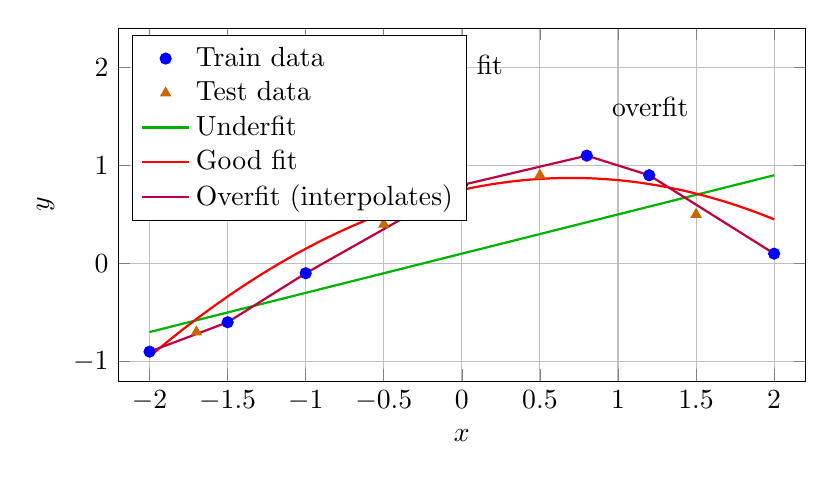
\begin{tikzpicture}
    \begin{axis}[
      width=0.85\textwidth,
      height=0.5\textwidth,
      xlabel={$x$},
      ylabel={$y$},
      legend style={at={(0.02,0.98)},anchor=north west},
      legend cell align=left,
      grid=major,
      xmin=-2.2, xmax=2.2,
      ymin=-1.2, ymax=2.4
    ]
      \addplot[only marks, mark=*, color=blue] coordinates {
        (-2,-0.9)
        (-1.5,-0.6)
        (-1,-0.1)
        (0,0.8)
        (0.8,1.1)
        (1.2,0.9)
        (2,0.1)
      };
      \addlegendentry{Train data}
      \addplot[only marks, mark=triangle*, color=orange!80!black] coordinates {
        (-1.7,-0.7)
        (-0.5,0.4)
        (0.5,0.9)
        (1.5,0.5)
      };
      \addlegendentry{Test data}
      \addplot[domain=-2:2, samples=50, thick, color=green!70!black] {0.1 + 0.4*x};
      \addlegendentry{Underfit}
      \addplot[domain=-2:2, samples=200, thick, color=red] {0.75 + 0.35*x - 0.25*x^2};
      \addlegendentry{Good fit}
      \addplot[thick, color=purple] coordinates {
        (-2,-0.9)
        (-1.5,-0.6)
        (-1,-0.1)
        (0,0.8)
        (0.8,1.1)
        (1.2,0.9)
        (2,0.1)
      };
      \addlegendentry{Overfit (interpolates)}

      \node[anchor=west] at (axis cs:-1.9,1.6) {underfit};
      \node[anchor=west] at (axis cs:-0.4,2.0) {good fit};
      \node[anchor=west] at (axis cs:0.9,1.6) {overfit};
    \end{axis}
  \end{tikzpicture}
\end{frame}

\begin{frame}{Model Complexity and Overfitting}
  \begin{itemize}
    \item Increasing degree increases flexibility and variance.
    \item Bias--variance tradeoff:
      \[
        \text{Error} = \text{Bias}^2 + \text{Variance} + \text{Noise}
      \]
    \item Overfitting: low training error, high test error.
  \end{itemize}
\end{frame}

\begin{frame}{Training vs.\ Test Error Curves}
  \centering
  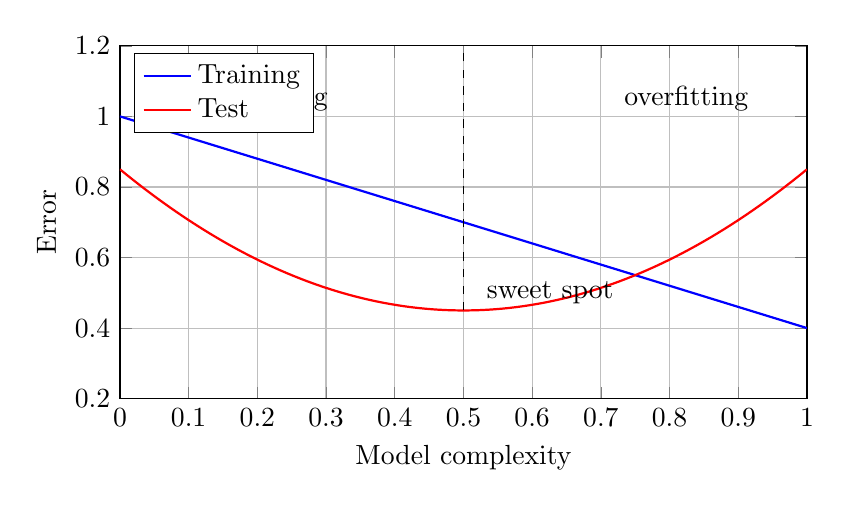
\begin{tikzpicture}
    \begin{axis}[
      width=0.85\textwidth,
      height=0.5\textwidth,
      xlabel={Model complexity},
      ylabel={Error},
      legend style={at={(0.02,0.98)},anchor=north west},
      legend cell align=left,
      grid=major,
      xmin=0, xmax=1,
      ymin=0.2, ymax=1.2
    ]
      \addplot[domain=0:1, samples=100, thick, color=blue] {0.9 - 0.6*x + 0.1};
      \addlegendentry{Training}
      \addplot[domain=0:1, samples=100, thick, color=red] {0.45 + 1.6*(x-0.5)^2};
      \addlegendentry{Test}
      \addplot[dashed, color=black] coordinates {(0.5,0.45) (0.5,1.2)};
      \node[anchor=west] at (axis cs:0.08,1.05) {underfitting};
      \node[anchor=west] at (axis cs:0.72,1.05) {overfitting};
      \node[anchor=west] at (axis cs:0.52,0.5) {sweet spot};
    \end{axis}
  \end{tikzpicture}
\end{frame}

\begin{frame}{Regularization: Motivation}
  \begin{itemize}
    \item Penalize complexity to improve generalization.
    \item Encourage simpler models with smaller coefficients.
    \item Trade-off controlled by \(\lambda\).
  \end{itemize}
\end{frame}

\begin{frame}{L2 Regularization (Ridge)}
  Objective:
  \[
    \min_{\boldsymbol{\theta}} \; \|X\boldsymbol{\theta} - \mathbf{y}\|_2^2 + \lambda \|\boldsymbol{\theta}\|_2^2
  \]
  Closed form:
  \[
    \boldsymbol{\theta}^* = (X^T X + \lambda I)^{-1} X^T \mathbf{y}
  \]
  Effect: shrinks coefficients toward zero.
\end{frame}

\begin{frame}{L1 Regularization (Lasso)}
  Objective:
  \[
    \min_{\boldsymbol{\theta}} \; \|X\boldsymbol{\theta} - \mathbf{y}\|_2^2 + \lambda \|\boldsymbol{\theta}\|_1
  \]
  \begin{itemize}
    \item Encourages sparse solutions.
    \item Performs implicit feature selection.
  \end{itemize}
\end{frame}

\begin{frame}{L1 vs.\ L2: Geometry}
  \centering
  \includegraphics[width=0.85\textwidth]{figs/regularization_l1_vs_l2.png}
\end{frame}

\begin{frame}{Summary}
  \begin{itemize}
    \item Linear regression = empirical risk minimization with MSE.
    \item Optimization via gradient descent or closed-form normal equations.
    \item Feature mappings enable nonlinear trends.
    \item Regularization controls overfitting.
  \end{itemize}
\end{frame}
